\begin{minipage}{.3\textwidth}
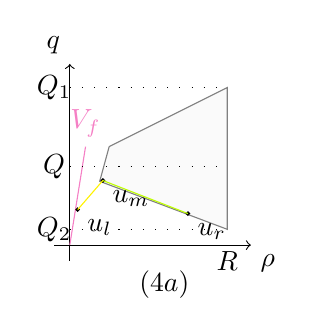
\begin{tikzpicture}
% coordinates
    \filldraw[fill=black!2, draw=black!50] plot [tension = 1] coordinates { (0.5,1.25) (2,2) (2,0.2) (0.38, 0.81) (0.5,1.25)};
    \draw[->] (0,-0.2) -- (0,2.3) node[anchor=south east] {$q$};
   
    \draw[magenta!50] (0,0) -- (0.2,1.25) node[anchor = south] {$V_f$};
    
    \filldraw[black] (1.5,0.4) circle (0.6pt) node[anchor = north west]{$u_r$} ;
    \filldraw[black] (0.42,0.82) circle (0.6pt) node[anchor = north west]{$u_m$} ;
    \filldraw[black] (0.1,0.45) circle (0.6pt) node[anchor = north west]{$u_l$} ;
    % \node at (1,1) {$\Omega_c$};
     \draw[->] (-0.2,0) -- (2.3,0) node[anchor=north west] {$\rho$};
    % \draw[-][black!50] (0, 0.98) -- (2, 0.2) node[anchor=south west] {$q_m(\rho)$} ;
    \node at (2,-0.2) {$R$};
     \node at (-0.2,2) {$Q_1$};
     \node at (-0.2,0.2) {$Q_2$};
     \node at (-0.2,1) {$Q$};
     \draw[loosely dotted] (0,1) -- (2,1);
     \draw[loosely dotted] (0,2) -- (2,2);
     \draw[loosely dotted] (0,0.2) -- (2,0.2);
     \node at (1.2,-0.5) {$(4a)$};
     % rarefactions and shocks
    %\draw[lime] (1.05, 1.33) -- (2, 1.6) ;
    %\draw[<-][cyan!50] (0.42, 1.19) -- (1, 1.33) ;
    
    %\draw[->][lime] (1.48,0.4)  -- (2, 0.2) ;
    \draw[lime] (0.42,0.82) -- (1.5,0.4)  ;
    \draw[yellow] (0.1,0.45) -- (0.42,0.82);
     
\end{tikzpicture}
\end{minipage}
\begin{minipage}{.3\textwidth}
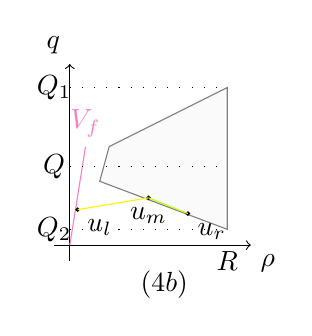
\begin{tikzpicture}
% coordinates
    \filldraw[fill=black!2, draw=black!50] plot [tension = 1] coordinates { (0.5,1.25) (2,2) (2,0.2) (0.38, 0.81) (0.5,1.25)};
    \draw[->] (0,-0.2) -- (0,2.3) node[anchor=south east] {$q$};
   
    \draw[magenta!50] (0,0) -- (0.2,1.25) node[anchor = south] {$V_f$};
    
    \filldraw[black] (1.5,0.4) circle (0.6pt) node[anchor = north west]{$u_r$} ;
    \filldraw[black] (1,0.6) circle (0.6pt) node[anchor = north]{$u_m$} ;
    \filldraw[black] (0.1,0.45) circle (0.6pt) node[anchor = north west]{$u_l$} ;
    % \node at (1,1) {$\Omega_c$};
     \draw[->] (-0.2,0) -- (2.3,0) node[anchor=north west] {$\rho$};
    % \draw[-][black!50] (0, 0.98) -- (2, 0.2) node[anchor=south west] {$q_m(\rho)$} ;
    \node at (2,-0.2) {$R$};
     \node at (-0.2,2) {$Q_1$};
     \node at (-0.2,0.2) {$Q_2$};
     \node at (-0.2,1) {$Q$};
     \draw[loosely dotted] (0,1) -- (2,1);
     \draw[loosely dotted] (0,2) -- (2,2);
     \draw[loosely dotted] (0,0.2) -- (2,0.2);
     \node at (1.2,-0.5) {$(4b)$};
     % rarefactions and shocks
    %\draw[lime] (1.05, 1.33) -- (2, 1.6) ;
    %\draw[<-][cyan!50] (0.42, 1.19) -- (1, 1.33) ;
    
    %\draw[->][lime] (1.48,0.4)  -- (2, 0.2) ;
    \draw[-][lime] (1,0.6) -- (1.5,0.4)  ;
    \draw[yellow] (0.1,0.45) -- (1,0.6);
     
\end{tikzpicture}
\end{minipage}
\begin{minipage}{.3\textwidth}
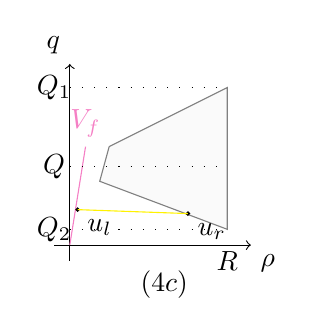
\begin{tikzpicture}
% coordinates
    \filldraw[fill=black!2, draw=black!50] plot [tension = 1] coordinates { (0.5,1.25) (2,2) (2,0.2) (0.38, 0.81) (0.5,1.25)};
    \draw[->] (0,-0.2) -- (0,2.3) node[anchor=south east] {$q$};
   
    \draw[magenta!50] (0,0) -- (0.2,1.25) node[anchor = south] {$V_f$};
    
    \filldraw[black] (1.5,0.4) circle (0.6pt) node[anchor = north west]{$u_r$} ;
    %\filldraw[black] (0.42,0.82) circle (0.6pt) node[anchor = north west]{$u_m$} ;
    \filldraw[black] (0.1,0.45) circle (0.6pt) node[anchor = north west]{$u_l$} ;
    % \node at (1,1) {$\Omega_c$};
     \draw[->] (-0.2,0) -- (2.3,0) node[anchor=north west] {$\rho$};
    % \draw[-][black!50] (0, 0.98) -- (2, 0.2) node[anchor=south west] {$q_m(\rho)$} ;
    \node at (2,-0.2) {$R$};
     \node at (-0.2,2) {$Q_1$};
     \node at (-0.2,0.2) {$Q_2$};
     \node at (-0.2,1) {$Q$};
     \draw[loosely dotted] (0,1) -- (2,1);
     \draw[loosely dotted] (0,2) -- (2,2);
     \draw[loosely dotted] (0,0.2) -- (2,0.2);
     \node at (1.2,-0.5) {$(4c)$};
     % rarefactions and shocks
    %\draw[lime] (1.05, 1.33) -- (2, 1.6) ;
    %\draw[<-][cyan!50] (0.42, 1.19) -- (1, 1.33) ;
    
    %\draw[->][lime] (1.48,0.4)  -- (2, 0.2) ;
    %\draw[-][cyan!50] (0.45,1.11) -- (1.5,1.45)  ;
    \draw[yellow] (0.1,0.45) -- (1.5,0.4);
     
\end{tikzpicture}
\end{minipage}